\documentclass[12pt]{article}

\usepackage{sbc-template}

\usepackage{graphicx,url}

\usepackage[brazil]{babel}
\usepackage[utf8]{inputenc}
%\usepackage[latin1]{inputenc}  

\sloppy

\title{Transmissão de Vídeo em Tempo Real em Redes Veiculares}

\author{Alfredo Goldman, Anderson Andrei, Patrick Abrahão }


\address{Instituto de Matemática e Estatística -- Universidade de São Paulo
  (USP)\\
  \email{\{gold\}@ime.usp.br, \{anderson.andrei.silva, patrick.menani\}@usp.br}
}

\begin{document} 

\maketitle

\begin{abstract}
In this paper we are interested in the context of live video streaming in mobile networks. Our goal is to realize an quantitative and qualitative analysis with the intent to better understand some aspects of data transmission. For such we analyzed some methods of package transmission of live video stream in this networks. We performed simulations to achieve a comparison between this methods in manner to classify them about their qualities and scalability. We performed comparisons between the protocols TCP, UDP and the transmission technique DASH, those simulations were made on OMNeT++ and INET Framework.
\end{abstract}
     
\begin{resumo} 
  Nesse artigo estamos interessados no contexto de transmissão de vídeo em tempo real entre dispositivos móveis. O nosso objetivo foi de realizar uma análise quantitativa e qualitativa com intuito de melhor entender alguns aspectos ligados à transmissão de dados.  Para tal analisamos algumas formas de transmissão de pacotes na rede para vídeo ao vivo. Realizamos simulações para chegarmos em comparações entre tais formas afim de classificá-las quanto sua qualidade e a escalabilidade na rede. As comparações foram feitas entre os protocolos TCP, UDP e a técnica de transmissão DASH através de simulações feitas no OMNeT++ e INET Framework.
\end{resumo}

\pagebreak

\section{General Information}

Estrutura:
	Motivação : "Estudo num ambiente de redes veículares."
    	"Cenário reduzido"
    Resumo
    Introdução
    	"No final dizer o que fizemos"
    Background conceitual
    	"Streaming de vídeo"
        "Dash"
        	"Youtube"
	Trabalhos relacionados
    	"Roger"
        "Edmundo"
        "Os de movimentação ou não"
	Experimental Settings
    	OMNET + INET
        Cenários Enumerar
        LinkGit
	Análise dos resultados
    	Mini conclusões sobre cada cenário enumerado
    Conclusões
    	Descobertas
        Visões futuras

\section{Introdução} \label{sec:introducao}
	
    Motivados pelo cenário de veículos autônomos desejamos estudar a transmissão de dados em redes compostas por tais. Com o crescimento da popularização da transmissão de vídeo ao vivo em redes sociais, serviços de entretenimento e outros, decidimos estudar tal vertente. Assim, estamos inseridos em um ambiente composto por uma estrutura capaz de fornecer dados de vídeo para veículos que trafegam em uma determinada área, e outra estrutura que configura o conjunto de veículos que utilizaram o serviço.
    Dada a complexidade de trabalhar com tal ambiente, em um primeiro momento, reduzimos nosso cenário de estudo para a segunda estrutura descrita assim como trabalharemos considerando dispositivos móveis e não veiculares.
    A parir desse cenário vamos estudar pontos de qualidade de serviço e de experiência do usuário para a transmissão de vídeo em tempo real. Vamos fazer comparações entre dois protocolos de transmissão e uma técnica aplicada em um deles. Os protocolos são o UDP e TCP, e a técnica é o DASH, aplicado no TCP. Obtendo dados dessas simulações vamos analisar deformação e perca de pacotes e perca de rotas.
    
\section{Background conceitual} \label{sec:conceitual}
	Componentes de redes veiculares
    AODV
    DASH
    Critérios de comparação
    Transmissao de video em tempo real

\section{Trabalhos relacionados} \label{sec:trabalhos}
\section{Cenários de experimentais} \label{sec:cenariosexp}
\section{Análise dos resultados} \label{sec:analise}
\section{Conslusão} \label{sec:conclusao}

\section{Figures and Captions}\label{sec:figs}

Figure and table captions should be centered if less than one line
(Figure~\ref{fig:exampleFig1}), otherwise justified and indented by 0.8cm on
both margins, as shown in Figure~\ref{fig:exampleFig2}. The caption font must
be Helvetica, 10 point, boldface, with 6 points of space before and after each
caption.

\begin{figure}[ht]
\centering
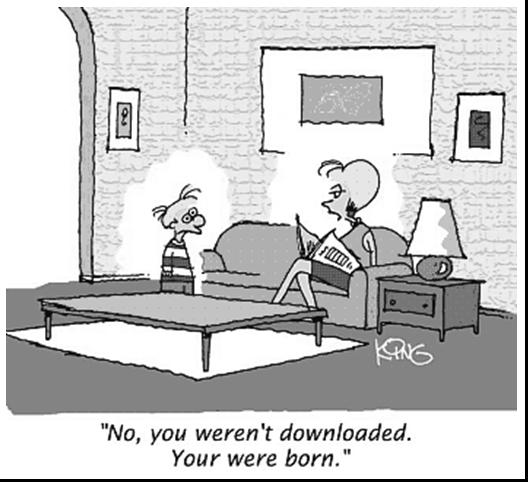
\includegraphics[width=.5\textwidth]{fig1.jpg}
\caption{A typical figure}
\label{fig:exampleFig1}
\end{figure}

\begin{figure}[ht]
\centering
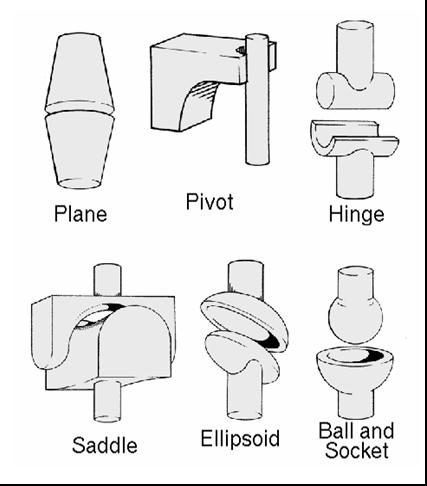
\includegraphics[width=.3\textwidth]{fig2.jpg}
\caption{This figure is an example of a figure caption taking more than one
  line and justified considering margins mentioned in Section~\ref{sec:figs}.}
\label{fig:exampleFig2}
\end{figure}

In tables, try to avoid the use of colored or shaded backgrounds, and avoid
thick, doubled, or unnecessary framing lines. When reporting empirical data,
do not use more decimal digits than warranted by their precision and
reproducibility. Table caption must be placed before the table (see Table 1)
and the font used must also be Helvetica, 10 point, boldface, with 6 points of
space before and after each caption.

\begin{table}[ht]
\centering
\caption{Variables to be considered on the evaluation of interaction
  techniques}
\label{tab:exTable1}
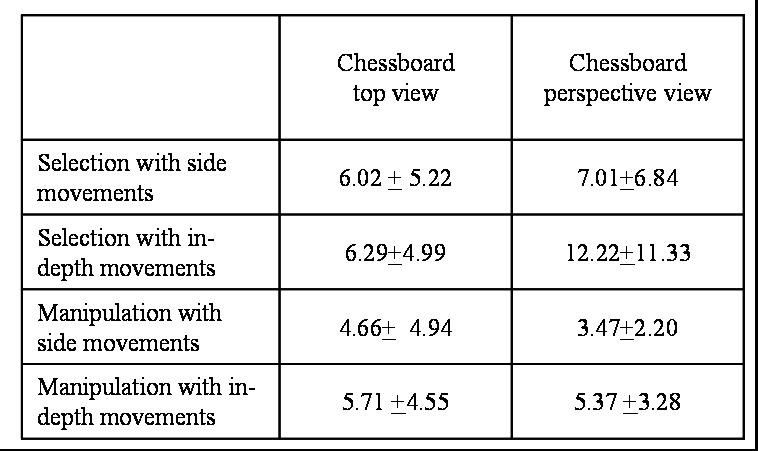
\includegraphics[width=.7\textwidth]{table.jpg}
\end{table}

\section{Images}

All images and illustrations should be in black-and-white, or gray tones,
excepting for the papers that will be electronically available (on CD-ROMs,
internet, etc.). The image resolution on paper should be about 600 dpi for
black-and-white images, and 150-300 dpi for grayscale images.  Do not include
images with excessive resolution, as they may take hours to print, without any
visible difference in the result. 

\section{References}

Bibliographic references must be unambiguous and uniform.  We recommend giving
the author names references in brackets, e.g. \cite{knuth:84},
\cite{boulic:91}, and \cite{smith:99}.

The references must be listed using 12 point font size, with 6 points of space
before each reference. The first line of each reference should not be
indented, while the subsequent should be indented by 0.5 cm.

\bibliographystyle{sbc}
\bibliography{sbc-template}

\end{document}
